\documentclass[12pt,draftclsnofoot,onecolumn]{IEEEtran}

\usepackage{comment,url}
\usepackage[dvips]{graphicx}
\usepackage{caption,subfig}
\usepackage{float}
\graphicspath{{../fig/}}
\DeclareGraphicsExtensions{.eps}
\usepackage{setspace}
\usepackage{amsmath}
\usepackage{amssymb}
\usepackage{cite}
\hyphenation{op-tical net-works semi-conduc-tor}

\usepackage{array}
\usepackage{mdwmath}
\usepackage{mdwtab}
\newtheorem{thm}{Theorem}
\doublespacing

\begin{document}

\title{On the Distribution of Random\\Distances in Rhombuses}

\author{Yanyan Zhuang~$^{\dagger *}$ and T. Aaron Gulliver~$^\ddagger$\\
$^\dagger$~University of British Columbia, Vancouver, BC, Canada\\
$^*$~New York University, New York, NY, USA\\
$^\ddagger$~University of Victoria, Victoria, BC, Canada}

\maketitle
\thispagestyle{empty}

\begin{abstract}
The distribution of random distances in geometric figures has important
applications in probability, statistics and many applied fields.
The study of the distribution of random distances in rhombuses is presented in this work.
Results are derived using an approach that is easier than those previous employed in the literature.
Explicit probability density functions are presented which are useful in a wide range of applications
such as operations research, road construction, and cellular signal transmission analysis.
\end{abstract}

\section{Introduction}
Rhombuses are one of the basic building blocks in two-dimensional tilings. The
distance distributions related to rhombuses have practical applications in a
wide range of fields, including urban transportation, operations research, and wireless communications.
Different from rectangles and squares, the point coordinates in rhombuses are not independent.
This paper presents a new and simple analytic approach that can be used
to deal with the dependency among point coordinates in rhombuses, and improves upon the results in~\cite{zhuang2011random}
and~\cite{zhuang2012geometrical}.
The analysis for rhombuses is extended to obtain similar results for regular hexagons, which
are widely used in planar tessellations in cellular
networks~\cite{zhuang2011geometric}, wireless ad-hoc
networks~\cite{zhuang2013planar}, wireless sensor
networks~\cite{schwiebert2001research, chang2008hexagonal, wang2009analytical},
and other networking applications~\cite{baltzis2012distance}.

In this work, results are derived for the distribution of
the random Euclidean distances within the same rhombus, between two parallel rhombuses
sharing a side, and between two rhombuses sharing a common diagonal.
% The approach used is easier to interpret than our prior
% work~\cite{zhuang2011random, zhuang2012geometrical}

\section{Related Work}

Planar tessellation, or tiling, is frequently used in many disciplines to divide
a surface, geographic region, or network, into clusters or cells using the repetition of a geometric figure.
Typical figures include triangles, squares, rhombuses and regular hexagons.
Hexagonal structures commonly appear in the fields of biology, chemistry, and astronomy, and
have inspired the design of honeycomb mesh networks~\cite{stojmenovic1997honeycomb}.
In cellular communication systems, a base station is usually located at the center of a cell which can be modeled as a hexagon.
If the base station uses directional antenna, then each cell sector is a rhombus.
%Closed-form distance distributions for hexagons were first presented in~\cite{zhuang2011random,zhuang2012geometrical}.

Ghosh was the first to derive the distance distributions for rectangles~\cite{ghosh1943distribution,ghosh1943random}.
Later, Alagar used the classic Crofton technique and its extensions to obtain the distribution of node distances
for circles and squares~\cite{alagar1976distribution}.
Mathai~\cite{mathai1998random,mathai1999random} and Sheng~\cite{sheng1985distance}
considered some simple geometric figures and analytically derived their distance distributions.
The methods employed, including local or global perturbations, differential equations and elementary statistical techniques,
either provide random distances from only a fixed point,
or yield results for very specific geometric figures that can be used in
planar tessellation~\cite{mathai1999introduction}.
Further, these approaches all assume that the coordinates of a point are independent.
For example, in a Cartesian system the $X$-coordinate of a point in a rectangle
is independent of the $Y$-coordinate, and in a polar coordinate
system, the radial and angular coordinates of a point are independent.

A method to obtain distance distributions in hexagons and rhombuses with interdependent point coordinates was
presented in~\cite{zhuang2011random,zhuang2012geometrical}.
However, the approach employed is quite complex.
In this work, a simple method is introduced which can be used to derive distance distributions in rhombuses.

\section{From Square to Rhombus}
For a rectangle with sides of lengths $a$ and $b$, define $X=x_1-x_2$ and
$Y=y_1-y_2$, where $(x_1, y_1)$ and $(x_2, y_2)$ are the coordinates of two
random points in the rectangle.
Assuming that $x_1, x_2 \in [0,a]$ and $y_1, y_2 \in [0, b]$ are uniformly and independently distributed,
$X$ and $Y$ have the following distributions
\begin{equation}\label{eq:fxy}
  f_X(x)=\frac{1}{a^2}\left\{
    \begin{array}{lr}
      a+x & -a\leq x \leq 0 \\
      a-x & 0 \leq x \leq a
    \end{array}
  \right.
  % \end{equation}
  % and
  % \begin{equation}
  ~~\mbox{ and }~~ f_Y(y)=\frac{1}{b^2}\left\{
    \begin{array}{lr}
      b+y & -b\leq y \leq 0 \\
      b-y & 0 \leq y \leq b
    \end{array}
  \right..
\end{equation}
%
Note that the distributions of $X$ and $Y$ are independent.
The distance between $(x_1, y_1)$ and $(x_2, y_2)$ is $D=\sqrt{X^2+Y^2}$.
Let the squared distance be $Z=D^2=X^2+Y^2$.
Then we have the distribution
\begin{eqnarray}\label{eq-rec}
F_Z(z)&=& {\rm P}\big(Z \leq z \big) = {\rm P}\big(X^2+Y^2 \leq z \big)\nonumber\\
%\iint F_{Z|X=x, Y=y}(z)f_{X,Y}(x,y){\rm d}x{\rm d}y\nonumber\\
%&=&\iint F\left(X^2+Y^2 \leq z\right|X=x, Y=y)f_{X,Y}(x,y){\rm d}x{\rm
%d}y\nonumber\\
&=&\iint_{\Omega_{\rm circle}}f_{X,Y}(x,y){\rm d}x{\rm d}y=
\iint_{\Omega_{\rm circle}}f_X(x)f_Y(y){\rm d}x{\rm d}y
\end{eqnarray}
where $\Omega_{\rm circle}=\left\{(X,Y)|X^2+Y^2\leq z, -a \leq X \leq a, -b \leq Y \leq b\right\}$
is the region of concentric circles of radius $\sqrt{z}$ satisfying $X^2+Y^2\leq z$
%(as the value of $z$ varies)
with joint pdf $f_X(x)f_Y(y)$ when neither $f_X(x)$ and $f_Y(y)$ is zero.
For example, $\Omega_{\rm circle}$ is shown in Figure~\ref{fig:square} for
$a=b=1$ and $f_X(x)$ and $f_Y(y)$ given in (\ref{eq:fxy}).
%with $0\leq z \leq1$ and $1\leq z \leq 2$.
%$X^2+Y^2 \leq z$ is the interior of a circle with radius $\sqrt{z}$, and
%$\Omega_{X^2+Y^2 \leq z}$ is the region where both $X^2+Y^2 \leq z$ and
%$f_X(x)f_Y(y)$ are non-zero.
The last equality in (\ref{eq-rec}) holds because the random variables
$X$ and $Y$ are independent in a rectangle.
Note that $X$ and $Y$ in (\ref{eq-rec}) correspond to the \textit{difference of the coordinates} of random points.
rather than the actual coordinates.
%
%Note that the region $\Omega_{X^2+Y^2 \leq z}$ is critical. It expresses the
%random variable $Z$ as a function of two other independent random variables
%$Z=X^2+Y^2$, and characterizes the distribution of $Z$, $P(Z\leq z)$, through
%$X$ and $Y$. The region $\Omega_{X^2+Y^2 \leq z}$ is therefore a projection
%of the surface of $X^2+Y^2 \leq z$, as $z$ varies, onto the
%$X$-$Y$ space where $f_X(x)f_Y(y)$ is non-zero.

\begin{figure}
  \centering
  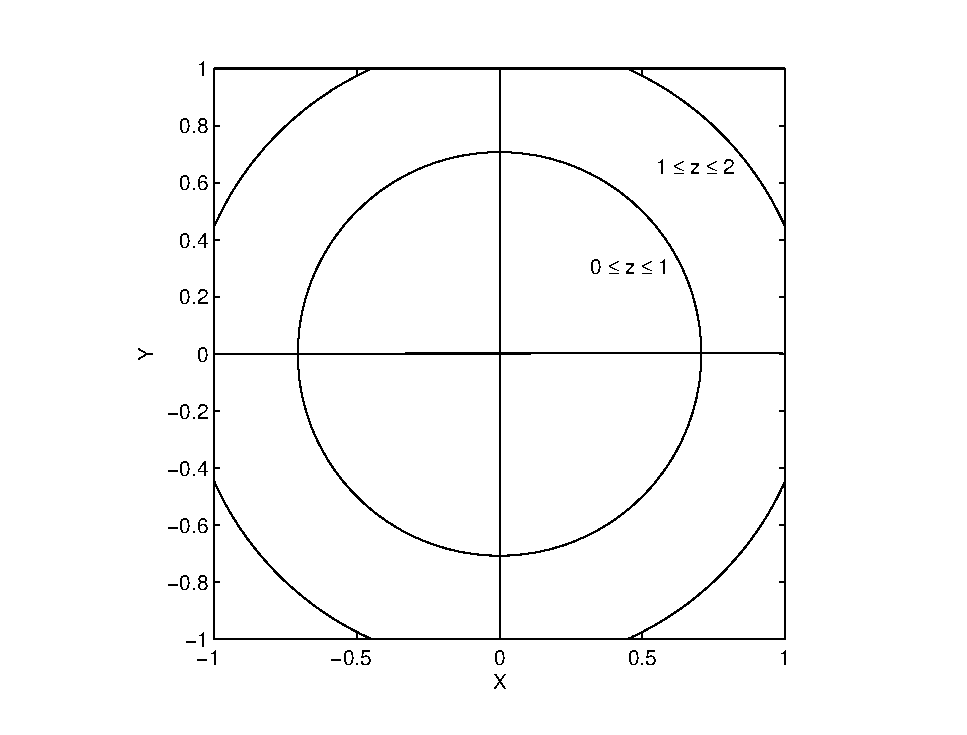
\includegraphics[width=0.5\columnwidth]{fig/square_within}
  \caption{Concentric circles $X^2+Y^2 \leq z$ for random distances in a unit square
  with $a=b=1$ in (\ref{eq:fxy}).}
  \label{fig:square}
\end{figure}

The interpretation of (\ref{eq-rec}) is similar to that in~\cite{ghosh1943distribution,
ghosh1943random} where the distance distributions for rectangles were derived.
Note that the formulation in (\ref{eq-rec}) improves on the approach
in~\cite{zhuang2011random, zhuang2012geometrical} as it simplifies the analysis.
As a special case, if $(x_1, y_1)$ and $(x_2, y_2)$ are located
in a unit square with $a=b=1$ in (\ref{eq:fxy}), then
\begin{equation}\label{eq:fxy-sqr}
  f_X(x)=\left\{
    \begin{array}{lr}
      1+x & -1\leq x \leq 0 \\
      1-x & 0 \leq x \leq 1
    \end{array}
  \right.
  % \end{equation}
  % and
  % \begin{equation}
  ~~\mbox{ and }~~ f_Y(y)=\left\{
    \begin{array}{lr}
      1+y & -1\leq y \leq 0 \\
      1-y & 0 \leq y \leq 1
    \end{array}
  \right..
\end{equation}
$\Omega_{\rm circle}$ in (\ref{eq-rec}) is then $\left\{(X,Y)|X^2+Y^2\leq z, -1 \leq X \leq 1, -1 \leq Y \leq 1\right\}$.
As shown in Figure~\ref{fig:square}, when $0\leq z\leq1$, the concentric circles corresponding to
$X^2+Y^2\leq z$ are entirely within the boundaries $x \in {[-1,1]}$ and $y \in {[-1,1]}$.
Since $X^2+Y^2\leq z$ is symmetric with respect to the $X=0$ and $Y=0$ axes, the
distribution of $Z$ is four times the distribution in the first quadrant where
$f_X(x)=1-x$ and $f_Y(y)=1-y$, giving
% where $0 \leq x \leq 1$ and $0 \leq y \leq 1$,
\begin{equation}\label{eq:f_z1}
F_Z(z)=4\iint_{\Omega_{\rm circle_1}}(1-x)(1-y){\rm d}x{\rm d}y,
\end{equation}
where $\Omega_{\rm circle_1}$ is the portion of $\Omega_{\rm circle}$ in
the first quadrant with $0 \leq X \leq 1$ and $0 \leq Y \leq 1$.
This is a much more general form than the expressions in~\cite{zhuang2011random,
zhuang2012geometrical}, and thus is more useful and easier to employ in deriving results, as will be shown in the next section.
The distribution of $Z$ when $0\leq z\leq1$ (and thus $0\leq d\leq1$), is
\begin{equation}
F_Z(z)=4\int_0^{\sqrt{z}}\int_0^{\sqrt{z-y^2}}(1-x){\rm d}x(1-y){\rm d}y
=\frac{z^2}{2}-\frac{8}{3}z^{3/2}+\pi z. \nonumber
\end{equation}

When $1\leq z\leq 2$ (or $1\leq d\leq\sqrt{2}$), the distribution can be obtained
similarly using (\ref{eq:f_z1}) (considering Figure~\ref{fig:square}), as
\begin{eqnarray}
F_Z(z)&=&4\left[\int_{0}^{1}\int_{0}^{\sqrt{z-1}}(1-x){\rm d}x(1-y){\rm
d}y+\int_{\sqrt{z-1}}^1\int_{0}^{\sqrt{z-y^2}}(1-x){\rm d}x(1-y){\rm d}y\right] \nonumber\\
&=&2z\left(\sin^{-1}\frac{1}{\sqrt{z}}-\sin^{-1}\sqrt{1-\frac{1}{z}}\right)+\frac{8z+4}{3}\sqrt{z-1}
-\frac{z^2}{2}-2z+3.\nonumber
\end{eqnarray}
%\end{small}
For $D=\sqrt{Z}$, the distance probability density function is
\begin{equation}\label{eq:fd-fz}
f_D(d)=F_Z'(d^2)=2df_Z(d^2),
\end{equation}
so that
\begin{equation}
  f_{D}(d)=\left\{
    \begin{array}{lr}
      2d(\pi-4d+d^2) & 0\leq d\leq 1\\
      2d[2\sin^{-1}(1/d)-2\sin^{-1}\sqrt{1-1/d^2}+4\sqrt{d^2-1}-d^2-2] & 1\leq d\leq \sqrt{2} \\
      0 & {\rm otherwise} \nonumber
    \end{array}
  \right..
\end{equation}
This is consistent with the results presented in~\cite{ghosh1943distribution} and \cite{ghosh1943random}.
%use and  can only express (\ref{eq:f_z1}) in explicit form.
%Similarly, in the next section (\ref{eq:within}), (\ref{eq:para}), (\ref{eq:fz_longdiag}) and
%(\ref{eq:fz_shortdiag}) are easily obtained using the general expression in (\ref{eq-rho}).

\section{Distribution of Random Distances in a Rhombus}\label{sec-withinr}

\begin{figure}
  \centering
  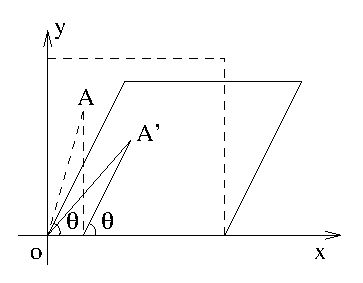
\includegraphics[width=0.4\columnwidth]{fig/single_rhombus}
  \caption{Random points in a rhombus.}
  \label{fig:rhombus}
\end{figure}

From Figure~\ref{fig:rhombus}, there is a linear relationship between a point $A
(x,y)$ in a square, and a point $A' (x',y')$ in a rhombus given by
\begin{equation}\label{eq:xr}
 \left\{
\begin{array}{lc}
x'=x+y\cos \theta \\
y'=y \sin \theta
\end{array}
\right.,
\end{equation}
where $\theta$ is the acute angle of the rhombus. In the following, we
assume both sides of the rhombus in Figure~\ref{fig:rhombus} are of unit
length and $\theta=\frac{\pi}{3}$, so that $x'=x+\frac{y}{2}$ and $y'=\frac{\sqrt{3}y}{2}$.

For two random points in a rhombus $(x_1',y_1')$ and $(x_2',y_2')$, define
$X'=x_1'-x_2'=\left(x_1-x_2\right)+\frac{1}{2}\left(y_1-y_2\right)=X+\frac{1}{2}
Y$, and
$Y'=y_1'-y_2'=\frac{\sqrt{3}}{2}\left(y_1-y_2\right)=\frac{\sqrt{3}}{2}Y$, where
$(x_1, y_1)$ and $(x_2, y_2)$ are the coordinates of two random points in a
unit square. $X$ and $Y$ have the same distribution as in
(\ref{eq:fxy-sqr}). The squared distance is $Z=D^2=X'^2+Y'^2=\left(X+\frac{1}{2}
Y\right)^2+\left(\frac{\sqrt{3}}{2}Y\right)^2=X^2+XY+Y^2$. Similar to
(\ref{eq-rec}), we have the distribution
\begin{eqnarray}\label{eq-rho}
F_Z(z)&=&{\rm P}\big(Z \leq z \big) = {\rm P}\big(X^2+XY+Y^2 \leq z \big)\nonumber\\
%\iint F\left(X^2+XY+Y^2 \leq z\right|X=x, Y=y)f_{X,Y}(x,y){\rm d}x{\rm
%d}y\nonumber\\
&=&\iint_{\Omega_{\rm ellipse}}f_{X,Y}(x,y){\rm d}x{\rm d}y=
\iint_{\Omega_{\rm ellipse}}f_X(x)f_Y(y){\rm d}x{\rm d}y,
\end{eqnarray}
where $\Omega_{\rm ellipse}=\left\{(X,Y)|X^2+XY+Y^2\leq z, x_{\rm L} \leq X \leq
x_{\rm H}, y_{\rm L}\leq Y \leq y_{\rm H}\right\}$ is the region of concentric ellipses
satisfying $X^2+XY+Y^2\leq z$
with semi-major axis of $\sqrt{2z}$ and semi-minor axis of $\sqrt{\frac{2z}{3}}$;
%(as the value of $z$ varies)
with joint pdf $f_X(x)f_Y(y)$, and $x_{\rm L} \leq X \leq x_{\rm H}, y_{\rm L}\leq
Y \leq y_{\rm H}$ is the region where neither $f_X(x)$ and $f_Y(y)$ is zero.
For example, $\Omega_{\rm ellipse}$ for the rhombus in Figure~\ref{fig:rhombus}
is shown in Figure~\ref{fig:z1}, where $x_{\rm L}=y_{\rm L}=-1, x_{\rm H}=y_{\rm H}=1$
as $X$ and $Y$ follow the distribution in (\ref{eq:fxy-sqr}).
%The intersection of  $X^2+XY+Y^2\leq z$ when $0\leq z \leq \frac{3}{4}$, $\frac{3}{4}\leq z \leq 1$,
%and $1\leq z \leq 3$, with $f_X(x)f_Y(y)$ is shown in Figure~\ref{fig:z1}.
%where $X^2+XY+Y^2 \leq z$ is the interior of an ellipse with semi-major axis
%equal to $\sqrt{2z}$, and semi-minor axis equal to $\sqrt{\frac{2z}{3}}$.
%$\Omega_{\rm ellipse}$ is the region where both $X^2+XY+Y^2 \leq z$ and
%$f_X(x)f_Y(y)$ are non-zero.
In the following, the subscript of $\Omega_{\rm ellipse}$ or $\Omega_{\rm circle}$ is
omitted when it is clear from the context.
Note that the formulation in (\ref{eq-rho}) is much simpler than that given in~\cite{zhuang2011random}
and~\cite{zhuang2012geometrical}.

\begin{figure}
  \centering
  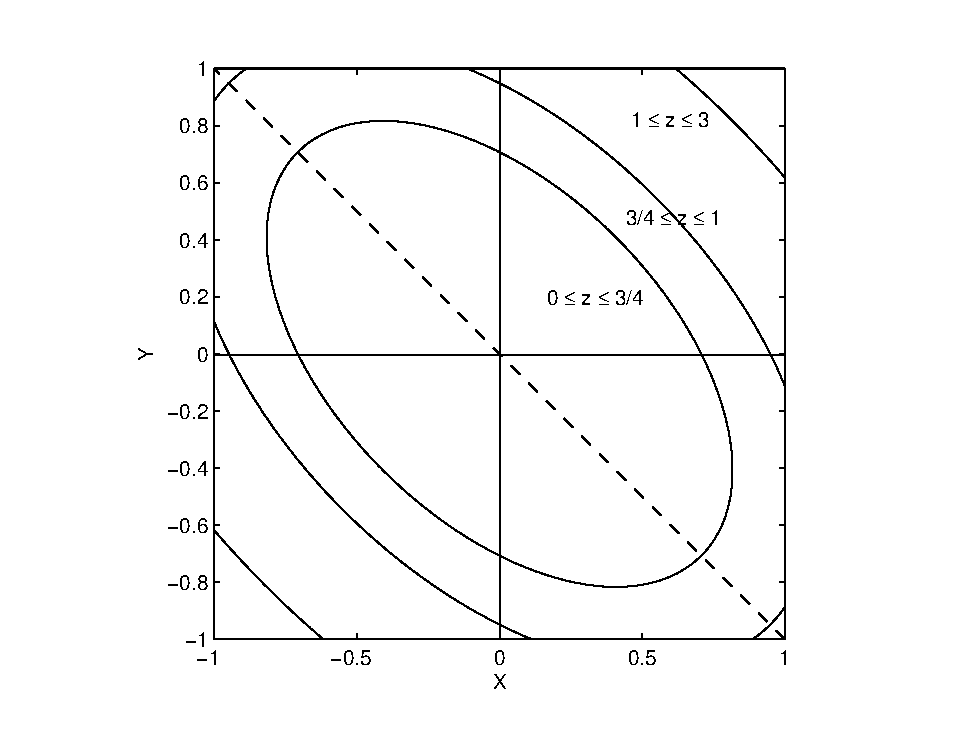
\includegraphics[width=0.5\columnwidth]{fig/rhombus_within}
  \caption{Concentric ellipses $X^2+XY+Y^2 \leq z$ for the random distances in a rhombus.}
  \label{fig:z1}
\end{figure}

From Figure~\ref{fig:z1}, the concentric ellipses $X^2+XY+Y^2 \leq z$ are symmetric with respect to $Y=-X$ and $Y=X$.
The distribution of $Z$ is therefore
\begin{equation}
\label{eq:within}
F_Z(z)=2\left[\iint_{\Omega_1}(1-x)(1-y){\rm d}x{\rm
d}y+\iint_{\Omega_2}(1-x)(1+y){\rm d}x{\rm d}y\right],
\end{equation}
where $\Omega_1$ is the portion of $\Omega_{\rm ellipse}$ in the first quadrant with
%is the interior of ellipse $X^2+XY+Y^2 \leq z$ with
$0 \leq X\leq 1$ and $0 \leq Y \leq 1$, and $\Omega_2$ is the portion of
$\Omega_{\rm ellipse}$ in the fourth quadrant when
%is the interior of this ellipse with
$0 \leq X \leq 1$ and $-1 \leq Y \leq 0$.
For example, consider Figure~\ref{fig:z1} with $0\leq z \leq \frac{3}{4}$ ($0\leq d\leq\frac{\sqrt{3}}{2}$).
$F_Z(z)$ can then be expressed as
\begin{small}
\begin{eqnarray}\label{eq:Z1_r_within}
F_Z(z)&=&2\left[\int_{0}^{\sqrt{z}}\int_{0}^{-\frac{y}{2}+\sqrt{z-\frac{3}{4}y^2
}}(1-x){\rm d}x(1-y){\rm
d}y+2\int_{-\sqrt{z}}^0\int_{-y}^{-\frac{y}{2}+\sqrt{z-\frac{3}{4}
y^2}}(1-x){\rm d}x(1+y){\rm d}y\right] \nonumber\\
&=&\left(\frac{2}{3}+\frac{\pi}{9\sqrt{3}}\right)z^2-\frac{32}{9}z^{3/2}+\frac{
2\pi}{\sqrt{3}}z.
\end{eqnarray}
\end{small}%

Note that in~\cite{zhuang2011random}
and~\cite{zhuang2012geometrical}, (\ref{eq:Z1_r_within}) was derived directly
for this specific case, which is a more complex approach than via the
more general expression in (\ref{eq:within}).
Similarly, the case when $\frac{3}{4} \leq z \leq 1$ ($\frac{\sqrt{3}}{2}\leq
d\leq 1$) and $1 \leq z \leq 3$ ($1\leq d\leq \sqrt{3}$) can
be derived according to (\ref{eq:within}) and Figure~\ref{fig:z1}.
Using (\ref{eq:fd-fz}), the probability density function of the random distances between two uniformly
distributed points that are both inside the same rhombus is
 \begin{equation}\label{eq:fd_r_within}
  f_{D_{\rm I}}(d)=2d\left\{
    \begin{array}{lr}

\left(\frac{4}{3}+\frac{2\pi}{9\sqrt{3}}\right)d^2-\frac{16}{3}d+\frac{2\pi}{
\sqrt{3}} & 0\leq d\leq \frac{\sqrt{3}}{2}\\

\frac{8}{\sqrt{3}}\left(1+\frac{d^2}{3}\right)\sin^{-1}\frac{\sqrt{3}}{2d}
+\left(\frac{4}{3}-\frac{10\pi}{9\sqrt{3}}\right)d^2-\frac{16}{3}d+\frac{10}{3}
\sqrt{4d^2-3}-\frac{2\pi}{\sqrt{3}} & \frac{\sqrt{3}}{2}\leq d\leq 1\\

\frac{4}{\sqrt{3}}\left(1-\frac{d^2}{3}\right)\sin^{-1}\frac{\sqrt{3}}{2d}
-\left(\frac{2}{3}-\frac{2\pi}{9\sqrt{3}}\right)d^2+\sqrt{4d^2-3}-\frac{2\pi}{
3\sqrt{3}}-1 & 1\leq d\leq \sqrt{3} \\

      0 & {\rm otherwise}
    \end{array}
  \right..
\end{equation}
This result was obtained in~\cite{zhuang2011random} and~\cite{zhuang2012geometrical} using
a much more complex and less intuitive approach.

\section{Distribution of Random Distances between Two Rhombuses}\label{sec-betweenr}

\begin{figure}
  \centering
  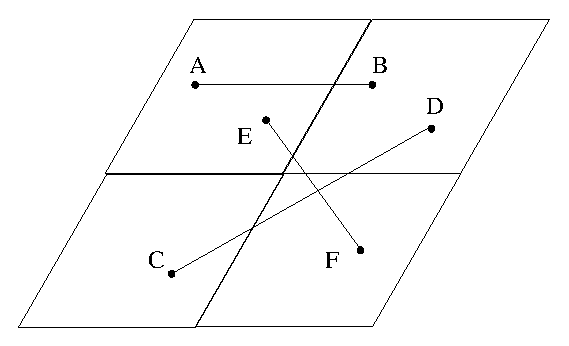
\includegraphics[width=0.4\columnwidth]{fig/rhombus}
  \caption{Random points in two rhombuses: $AB$ --- two parallel rhombuses
  sharing a side; $CD$ --- two rhombuses sharing a common \textit{long}
  diagonal; $EF$ --- two rhombuses sharing a common \textit{short} diagonal.}
  \label{fig:two}
\end{figure}

In addition to two points in the same rhombus, one can have points in two parallel rhombuses
sharing a side such as $AB$ in Figure~\ref{fig:two}, and points in two
rhombuses sharing a common diagonal such as $CD$ and $EF$ in Figure~\ref{fig:two}.
Here $CD$ and $EF$ are two different cases, and in the following, they are referred to
as long diagonal (long-diag) and short diagonal (short-diag), respectively.

\subsection{Distribution of Random Distances between Two Parallel Rhombuses Sharing a Side}

For $AB$ in Figure~\ref{fig:two}, the distributions of $X$ and $Y$ are
\begin{equation}\label{eq:fxy_para}
  f_X(x)=\left\{
    \begin{array}{lr}
      x & 0\leq x \leq 1 \\
      2-x & 1 \leq x \leq 2
    \end{array}
  \right.,
  ~~\mbox{ and }~~ f_Y(y)=\left\{
    \begin{array}{lr}
      1+y & -1\leq y \leq 0 \\
      1-y & 0 \leq y \leq 1
    \end{array}
  \right.,
\end{equation}
respectively.
The distribution of $Z$ is the same as in (\ref{eq-rho}), with
$f_X(x)$ and $f_Y(y)$ as above.
Therefore, $\Omega_{\rm ellipse}$ %in (\ref{eq-rho})
is the region of concentric ellipses satisfying $X^2+XY+Y^2 \leq z$ with $0 \leq X \leq 2$ and $-1\leq Y \leq 1$,
%when $0\leq z \leq \frac{3}{4}$, $\frac{3}{4}\leq z \leq 1$, $1\leq z \leq 2$, $3\leq z
%\leq 4$, and $4\leq z \leq 7$,
%$x_{\rm L}=0, x_{\rm H}=2, y_{\rm L}=y_{\rm H}=1$,
as shown in Figure~\ref{fig:para}.
Note that the concentric ellipses are the same as in Figure~\ref{fig:z1},
and only the non-zero region of $f_X(x)f_Y(y)$, as indicated in (\ref{eq:fxy_para}), is different.
This gives
\begin{eqnarray}\label{eq:para}
 F_Z(z)&=&\iint_{\Omega_1}x(1+y){\rm d}x{\rm d}y+\iint_{\Omega_2}x(1-y){\rm
d}x{\rm d}y\nonumber \\
&&+\iint_{\Omega_3}(2-x)(1+y){\rm d}x{\rm d}y+\iint_{\Omega_4}(2-x)(1-y){\rm
d}x{\rm d}y,
\end{eqnarray}
where $\Omega_1$ is the interior of the ellipses $X^2+XY+Y^2 \leq z$ with $0 \leq X
\leq 1$ and $-1 \leq Y \leq 0$, $\Omega_2$ is the interior of the ellipses
with $0 \leq X \leq 1$, $0 \leq Y \leq 1$, and $\Omega_3$ and $\Omega_4$ exist only when
$1 \leq X \leq 2$ and $-1 \leq Y \leq 0$ and $1 \leq X \leq 2$ and $0 \leq Y \leq 1$, respectively.
% where $\Omega_1$ to $\Omega_4$ are the interior of ellipse $X^2+XY+Y^2 \leq z$
% in four different quadrants, respectively.
As shown in Figure~\ref{fig:para}, depending on the value of $z$, not all four regions
$\Omega_1$ to $\Omega_4$ will exist in (\ref{eq:para}).
For example, when $0\leq z \leq \frac{3}{4}$ ($0\leq d\leq \frac{\sqrt{3}}{2}$), $\Omega_3$ and $\Omega_4$
do not exist. $F_Z(z)$ in this case is
\begin{small}
\begin{eqnarray}\label{eq:Z1_r_para}
 F_Z(z)&=&\left[\int_0^{\sqrt{\frac{4z}{3}}}\int_{-\frac{x}{2}-\sqrt{z-\frac{3}{
4}x^2}}^{-\sqrt{\frac{z}{3}}}(1+y){\rm d}yx{\rm d}x+\int_{-\sqrt{\frac{z}{3}}}
^0\int_0^{-\frac{y}{2}+\sqrt{z-\frac{3}{4}y^2}}x{\rm d}x(1+y){\rm d}y\right]
\nonumber\\
&&+\int_0^{\sqrt{z}}\int_0^{-\frac{y}{2}+\sqrt{z-\frac{3}{4}y^2}}
x{\rm d}x(1-y){\rm
d}y=\frac{8}{9}z^{3/2}-\left(\frac{1}{3}+\frac{\pi}{18\sqrt{3}}
\right)z^2.
\end{eqnarray}
\end{small}

\begin{figure}
  \centering
  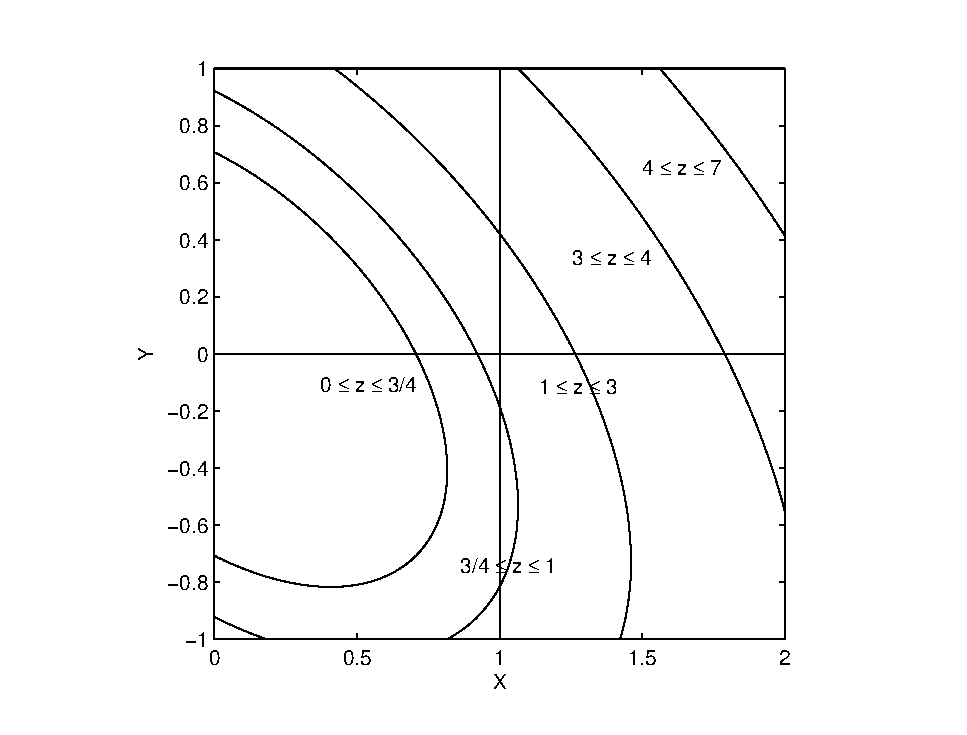
\includegraphics[width=0.5\columnwidth]{fig/rhombus_para}
  \caption{Concentric ellipses satisfying $X^2+XY+Y^2 \leq z$ for random distances between two parallel rhombuses sharing a side.}
  \label{fig:para}
\end{figure}

Note that in~\cite{zhuang2011random}
and~\cite{zhuang2012geometrical}, (\ref{eq:Z1_r_para}) was derived for just this particular case.
This is much more difficult than employing the more general expression given in (\ref{eq:para}).
Similarly, the case when $\frac{3}{4} \leq z \leq 1$ ($\frac{\sqrt{3}}{2}\leq
d\leq 1$), $1 \leq z \leq 3$ ($1\leq d\leq \sqrt{3}$), $3 \leq z \leq 4$ ($\sqrt{3}\leq
d\leq 2$), and $4 \leq z \leq 7$ ($2\leq d\leq \sqrt{7}$) can
easily be derived from (\ref{eq:para}) and Figure~\ref{fig:para}.
Using an approach similar to that above with (\ref{eq:fd-fz}), the probability density
function of the random distances between two uniformly distributed points, one
in each of two adjacent rhombuses that are parallel and sharing a side is
\begin{small}
 \begin{equation}\label{eq:fd_r_para}
  f_{D_{\rm P}}(d)=2d\left\{
    \begin{array}{lr}

\frac{4}{3}d-\left(\frac{2}{3}+\frac{\pi}{9\sqrt{3}}\right)d^2 & 0\leq d\leq
\frac{\sqrt{3}}{2}\\

-\frac{2}{\sqrt{3}}(d^2+2)\sin^{-1}\frac{\sqrt{3}}{2d}+\left(\frac{8\pi}
{9\sqrt{3}}-\frac{2}{3}\right)d^2+\frac{4}{3}d-\frac{11}{6}\sqrt{4d^2-3}+\frac{
2\pi}{\sqrt{3}} & \frac{\sqrt{3}}{2}\leq d\leq 1\\

\frac{4d^2}{3\sqrt{3}}\sin^{-1}\frac{\sqrt{3}}{2d}+\left(\frac{2}{3}
-\frac{2\pi}{9\sqrt{3}}\right)d^2-\frac{8}{3}d+\frac{\sqrt{4d^2-3}}{3}+\frac{
2\pi}{3\sqrt{3}}+\frac{1}{2} & 1\leq d\leq \sqrt{3} \\

\left(\frac{2}{\sqrt{3}}-\frac{d^2}{3\sqrt{3}}\right)\sin^{-1}\frac{\sqrt
{3}}{2d}+\left(\frac{2}{\sqrt{3}}+\frac{d^2}{3\sqrt{3}}\right)\sin^{-1}\frac{
\sqrt{3}}{d}+\left(\frac{1}{3}-\frac{\pi}{9\sqrt{3}}\right)d^2 \\
~~~~-\frac{8}{3}d+\frac{7}{12}\sqrt{4d^2-3}+\sqrt{d^2-3}+\frac{3}{4}
-\frac{2\pi}{3\sqrt{3}} & \sqrt{3}\leq d\leq 2 \\

\left(\frac{2}{\sqrt{3}}-\frac{d^2}{3\sqrt{3}}\right)\left(\sin^{-1}\frac{
\sqrt{3}}{2d}+\sin^{-1}\frac{\sqrt{3}}{d}\right)+\left(\frac{\pi}{9\sqrt{3}}
-\frac{1}{3 }\right)d^2 \\
~~~~+\frac{7}{12}\sqrt{4d^2-3}+\frac{\sqrt{d^2-3}}{3}-\frac{2\pi}{3\sqrt{3}}
-\frac{5}{4} & 2 \leq d \leq \sqrt{7} \\

      0 & {\rm otherwise}
    \end{array}
 \right..
\end{equation}
\end{small}

\subsection{Distribution of Random Distances between Two Long-Diag Rhombuses}

For $CD$ in Figure~\ref{fig:two}, the distributions of $X$ and $Y$ are
\begin{equation}\label{eq:fxy_diag}
  f_X(x)=\left\{
    \begin{array}{lr}
      x & 0\leq x \leq 1 \\
      2-x & 1 \leq x \leq 2
    \end{array}
  \right.,
  ~~\mbox{ and }~~ f_Y(y)=\left\{
    \begin{array}{lr}
      y & 0\leq y \leq 1 \\
      2-y & 1 \leq y \leq 2
    \end{array}
  \right.,
\end{equation}
respectively.
Therefore, $\Omega_{\rm ellipse}$ in (\ref{eq-rho}) is the
region of concentric ellipses satisfying $X^2+XY+Y^2 \leq z$ with $0 \leq X \leq 2, 0\leq Y \leq 2$,
as shown in Figure~\ref{fig:diag1}.
%The intersection of ellipses $X^2+XY+Y^2 \leq z$
%when $0\leq z \leq 1$, $1\leq z \leq 3$, $3\leq z \leq 4$, $4\leq z
%\leq 7$, and $7\leq z \leq 12$, with $f_X(x)f_Y(y)$ is shown in
%Figure~\ref{fig:diag1}.
Note that the concentric ellipses are the same as those in Figure~\ref{fig:z1}, and only the non-zero
region of $f_X(x)f_Y(y)$, as indicated in (\ref{eq:fxy_diag}), is different.
As these concentric ellipses are symmetric with respect to $Y=X$, the distribution of $Z$ is
\begin{equation}\label{eq:fz_longdiag}
 F_Z(z)=\iint_{\Omega_1}xy{\rm d}x{\rm d}y+2\iint_{\Omega_2}x(2-y){\rm d}x{\rm
d}y+\iint_{\Omega_3}(2-x)(2-y){\rm d}x{\rm d}y,
\end{equation}
where $\Omega_1$ is the interior of the ellipses $X^2+XY+Y^2 \leq z$ with $0 \leq X
\leq 1$ and $0 \leq Y \leq 1$, $\Omega_2$ is the interior of the ellipses with
$0 \leq X \leq 1$ and $1 \leq Y \leq 2$, and $\Omega_3$ exists only when $1 \leq X \leq 2$
and $1 \leq Y \leq 2$.
For example, when $0\leq z \leq 1$ ($0\leq d \leq 1$), only $\Omega_1$
exists as shown in Figure~\ref{fig:diag1}, thus
\begin{small}
 \begin{equation}
 F_Z(z)=\int_0^{\sqrt{z}}\int_0^{-\frac{y}{2}+\sqrt{z-\frac{3}{4}y^2}}
x{\rm d}xy{\rm d}y=\left(\frac{1}{6}-\frac{\pi}{18\sqrt{3}}\right)z^2.
\end{equation}
\end{small}

\begin{figure}
  \centering
  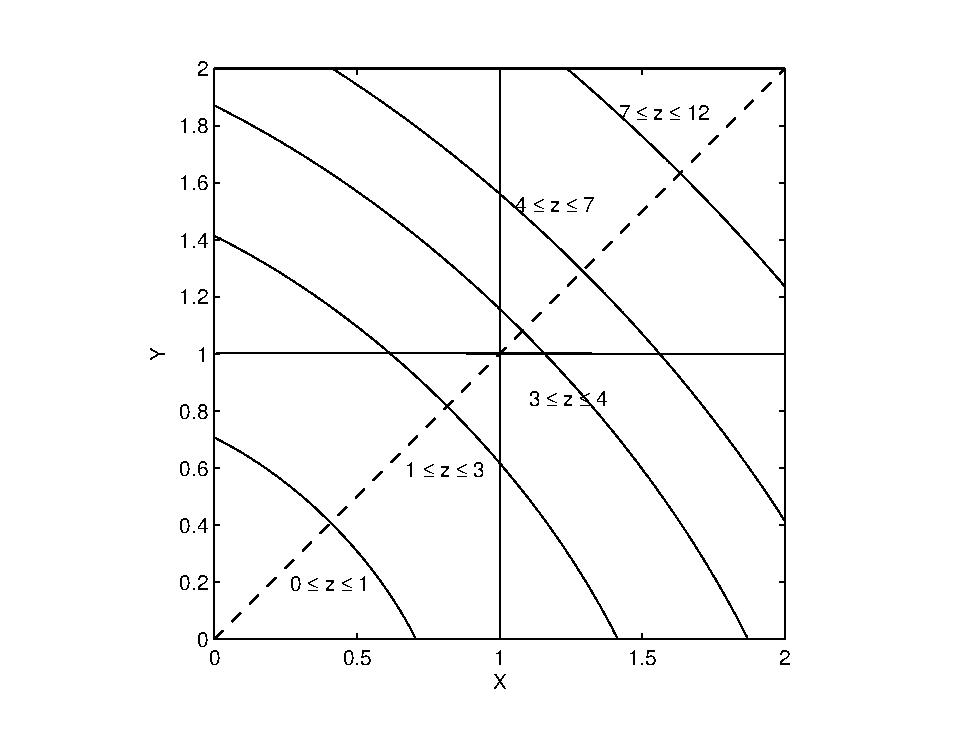
\includegraphics[width=0.5\columnwidth]{fig/rhombus_diag1}
  \caption{Concentric ellipses satisfying $X^2+XY+Y^2 \leq z$ for random distances between two long-diag rhombuses.}
  \label{fig:diag1}
\end{figure}

Similarly, the case when $1 \leq z \leq 3$ ($1\leq d\leq \sqrt{3}$),
$3 \leq z \leq 4$ ($\sqrt{3}\leq d\leq 2$), $4 \leq z \leq 7$ ($2\leq d\leq
\sqrt{7}$) and $7 \leq z \leq 12$ ($\sqrt{7}\leq d\leq 2\sqrt{3}$) can
be derived from (\ref{eq:fz_longdiag}) and Figure~\ref{fig:diag1}.
Therefore, the probability density function of the random distances between two
uniformly distributed points, one in each of two adjacent rhombuses sharing
a common long diagonal is
\begin{small}
\begin{equation}\label{eq:fd_r_diag1}
  f_{D_{\rm LD}}(d)=2d\left\{
    \begin{array}{lr}

\left(\frac{1}{3}-\frac{\pi}{9\sqrt{3}}\right)d^2 & 0\leq d\leq 1\\

-\frac{4d^2}{3\sqrt{3}}\sin^{-1}\frac{\sqrt{3}}{2d}+\left(\frac{\pi}{3\sqrt{3}}
-1\right)d^2+\frac{8}{3}d-\frac{\sqrt{4d^2-3}}{3}-1 & 1\leq d\leq \sqrt{3}\\

\frac{4}{\sqrt{3}}\left(\frac{d^2}{3}-2\right)\sin^{-1}\frac{\sqrt{3
}}{2d}+\left(\frac{1}{3}-\frac{\pi}{9\sqrt{3}}\right)d^2+\frac{8}{3}d-\frac{7}{3
}\sqrt{4d^2-3}+\frac{4\pi}{3\sqrt{3}}+1 & \sqrt{3}\leq d\leq 2\\

\frac{4}{\sqrt{3}}\left(\frac{d^2}{3}-2\right)\sin^{-1}\frac{\sqrt{3
}}{2d}+\frac{2d^2}{3\sqrt{3}}\sin^{-1}\frac{\sqrt{3}}{d}+\left(1-\frac{\pi}{
3\sqrt{3}}\right)d^2 \\
~~~~-\frac{7}{3}\sqrt{4d^2-3}+\frac{2}{3}\sqrt{d^2-3}+\frac{4\pi}{3\sqrt{3}}+3 &
2\leq d\leq \sqrt{7} \\

\frac{2}{\sqrt{3}}\left(4-\frac{d^2}{3}\right)\sin^{-1}\frac{\sqrt{3}}{d}
+\left(\frac{\pi}{9\sqrt{3}}-\frac{1}{3}\right)d^2+2\sqrt{d^2-3}-\frac{4\pi}{
3\sqrt{3}}-2 & \sqrt{7} \leq d \leq 2\sqrt{3} \\

      0 & {\rm otherwise}
    \end{array}
  \right..
\end{equation}
\end{small}

\subsection{Distribution of Random Distances between Two Short-Diag Rhombuses}

\begin{figure}
  \centering
  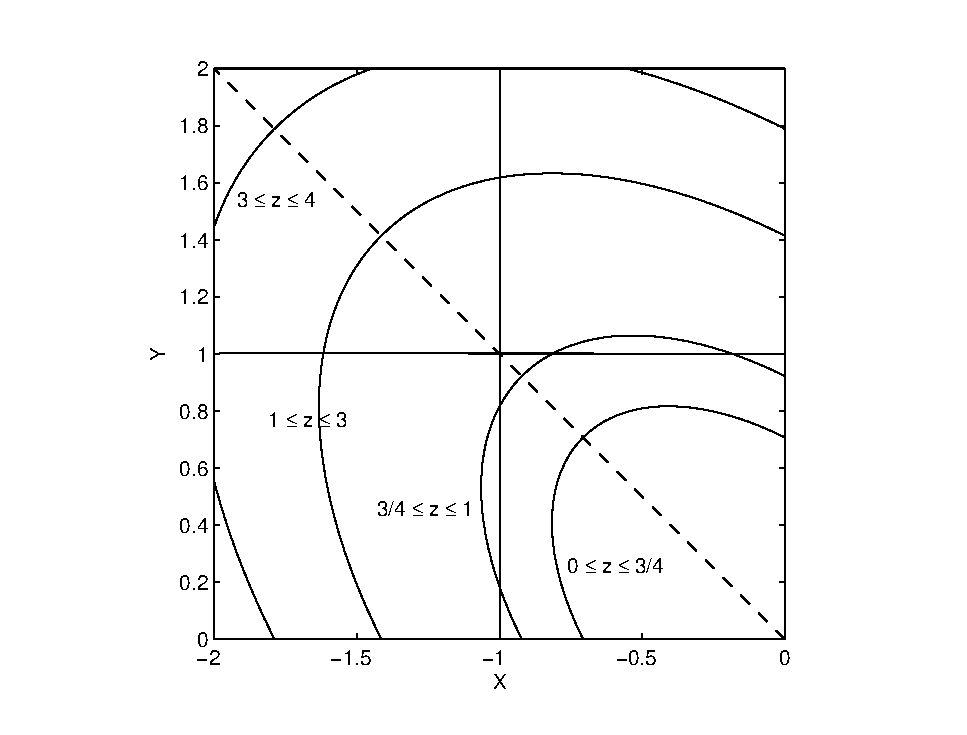
\includegraphics[width=0.5\columnwidth]{fig/rhombus_diag2}
  \caption{Concentric ellipses satisfying $X^2+XY+Y^2 \leq z$ for random distances between two short-diag rhombuses.}
  \label{fig:diag2}
\end{figure}

For $EF$ in Figure~\ref{fig:two}, the distributions of $X$ and $Y$ are
\begin{equation}\label{eq:fxy_diag2}
  f_X(x)=\left\{
    \begin{array}{lr}
      2+x & -2\leq x \leq -1 \\
      -x & -1 \leq x \leq 0
    \end{array}
  \right.,
  ~~\mbox{ and }~~ f_Y(y)=\left\{
    \begin{array}{lr}
      y & 0\leq y \leq 1 \\
      2-y & 1 \leq y \leq 2
    \end{array}
  \right.,
\end{equation}
respectively.
Therefore, $\Omega_{\rm ellipse}$ in (\ref{eq-rho})
is the region of concentric ellipses satisfying $X^2+XY+Y^2 \leq z$ with $-2 \leq X \leq 0,
0\leq Y \leq 2$, as shown in Figure~\ref{fig:diag2}.
%The intersection of ellipses $X^2+XY+Y^2 \leq z$
%when $0\leq z \leq \frac{3}{4}$, $ \frac{3}{4}\leq z \leq 1$, $1\leq z
%\leq 3$, and $3\leq z \leq 4$, with $f_X(x)f_Y(y)$ is shown in
%Figure~\ref{fig:diag2}.
Note that these concentric ellipses are
the same as those in Figure~\ref{fig:z1}, and only the non-zero
region of $f_X(x)f_Y(y)$, as indicated in (\ref{eq:fxy_diag2}),
is different
%The ellipse $X^2+XY+Y^2 \leq z$ is shown in Figure~\ref{fig:diag2}.
As the ellipse is symmetric with respect to $Y=-X$, the distribution of $Z$ is
\begin{equation}
\label{eq:fz_shortdiag}
 F_Z(z)=\iint_{\Omega_1}(-x)y{\rm d}x{\rm d}y+2\iint_{\Omega_2}(-x)(2-y){\rm
d}x{\rm d}y+\iint_{\Omega_3}(2+x)(2-y){\rm d}x{\rm d}y,
\end{equation}
where $\Omega_1$ is the interior of the ellipses $X^2+XY+Y^2 \leq z$ with $-1 \leq X
\leq 0$ and $0 \leq Y \leq 1$, $\Omega_2$ is the interior of the ellipses with
$-1 \leq X \leq 0$ and $1 \leq Y \leq 2$, and $\Omega_3$ exists only when $-2 \leq X \leq
-1$ and $1 \leq Y \leq 2$.
For example, when $\frac{3}{4} \leq z \leq 1$ ($\frac{\sqrt{3}}{2} \leq d \leq 1$),
$\Omega_3$ does not exist so the distribution of $Z$ is
\begin{small}
 \begin{eqnarray}\label{eq:Z2_r_diag2}
 F_Z(z)&=&\left[2\int_{-\sqrt{z}}^0\int_{-x}^{-\frac{x}{2}+\sqrt{z-\frac{3}{4}
x^2}}y{\rm d}y(-x){\rm
d}x-2\int_{-\frac{1}{2}-\sqrt{z-\frac{3}{4}}}^{-\frac{1}{2}+\sqrt{
z-\frac{3}{4}}}\int_1^{-\frac{x}{2}+\sqrt{z-\frac{3}{4}x^2}}y{\rm d}y(-x){\rm
d}x\right] \nonumber\\
&&+2\int_{-\frac{1}{2}-\sqrt{z-\frac{3}{4}}}^{-\frac{1}{2}+\sqrt{z-\frac{3}{4}}}
\int_1^{-\frac{x}{2}+\sqrt{z-\frac{3}{4}x^2}}(2-y){\rm d}y(-x){\rm d}x
\nonumber\\
&=&-\frac{2z^2}{3\sqrt{3}}\sin^{-1}\frac{\sqrt{3}}{2}\frac{\sqrt{4z-3}}{z}
+\left(\frac{1}{6}+\frac{\pi}{9\sqrt{3}}\right)z^2+\frac{10z-3}{18}\sqrt{4z-3}.
\end{eqnarray}
\end{small}

Similarly, the case when $0 \leq z \leq \frac{3}{4}$ ($0\leq d\leq
\frac{\sqrt{3}}{2}$), $1 \leq z \leq 3$ ($1\leq d\leq \sqrt{3}$) and
$3 \leq z \leq 4$ ($\sqrt{3}\leq d\leq 2$) can be derived from (\ref{eq:fz_shortdiag}) and Figure~\ref{fig:diag2}.
The probability density function of the random distances between two uniformly
distributed points, one in each of two adjacent rhombuses sharing a common
short diagonal is
\begin{small}
\begin{equation}\label{eq:fd_r_diag2}
  f_{D_{\rm SD}}(d)=2d\left\{
    \begin{array}{lr}

\left(\frac{1}{3}+\frac{2\pi}{9\sqrt{3}}\right)d^2 & 0\leq d\leq
\frac{\sqrt{3}}{2}\\

\frac{8d^2}{3\sqrt{3}}\sin^{-1}\frac{\sqrt{3}}{2d}+\left(\frac{1}{3}-\frac{10\pi
}{9\sqrt{3}}\right)d^2+\frac{2}{3}\sqrt{4d^2-3} & \frac{\sqrt{3}}{2} \leq d \leq
1\\

-\left(\frac{4d^2}{3\sqrt{3}}+\frac{8}{\sqrt{3}}\right)\sin^{-1}\frac{\sqrt{3}}{
2d}+\left(\frac{1}{3}+\frac{2\pi}{9\sqrt{3}}\right)d^2+\frac{8}{3}d-3\sqrt{
4d^2-3}+\frac{8\pi}{3\sqrt{3}}+1 & 1\leq d\leq \sqrt{3} \\

\frac{8}{\sqrt{3}}\sin^{-1}\frac{\sqrt{3}}{d}-d^2+\frac{8}{3}d+\frac{8}{3}\sqrt{
d^2-3}-\frac{8\pi}{3\sqrt{3}}-4 & \sqrt{3}\leq d\leq 2 \\

      0 & {\rm otherwise}
    \end{array}
  \right..
\end{equation}
\end{small}

Equations (\ref{eq:fd_r_para}), (\ref{eq:fd_r_diag1}) and
(\ref{eq:fd_r_diag2}) were derived in~\cite{zhuang2011random}
and~\cite{zhuang2012geometrical} using a much more complex approach.
Conversely, the intermediate results given in (\ref{eq:within}), (\ref{eq:para}),
(\ref{eq:fz_longdiag}) and (\ref{eq:fz_shortdiag}) are easily obtained using (\ref{eq-rho}).

\section{Validation}

\begin{figure}
  \centering
  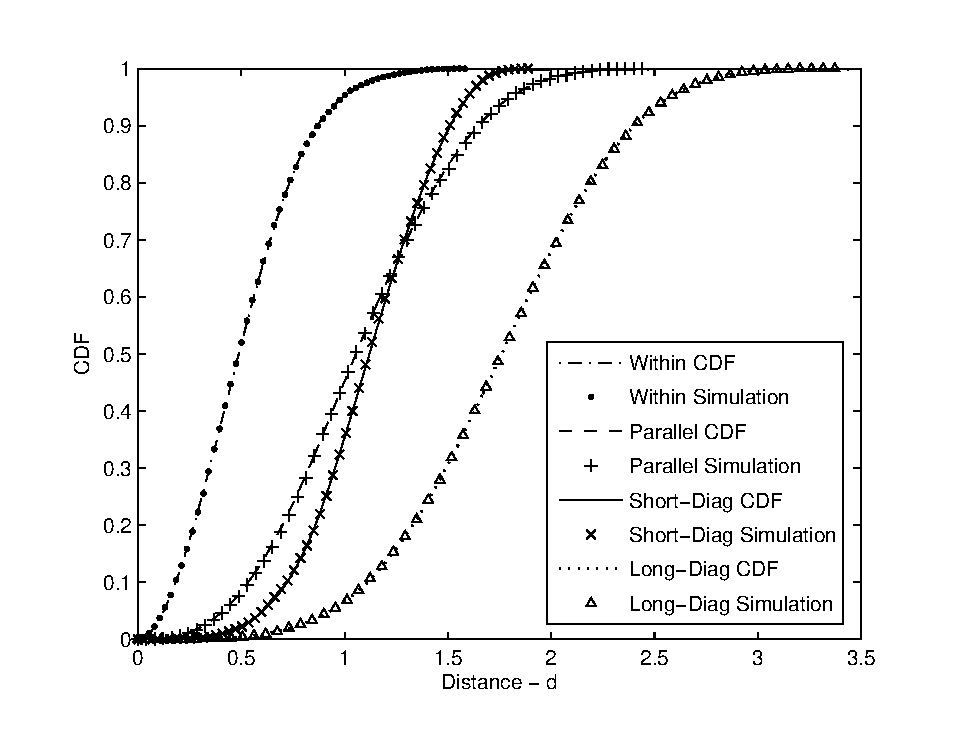
\includegraphics[width=0.6\columnwidth]{fig/rhombus_cdf}
  \caption{Cumulative distribution functions and simulation results for the
  distribution of random distances in rhombuses.}
  \label{fig:cdf}
\end{figure}

Figure~\ref{fig:cdf} shows the cumulative
distribution functions (CDFs) of the random distances
in rhombuses derived in Sections~\ref{sec-withinr} and \ref{sec-betweenr},
and the results obtained by generating $1,000$ pairs of random points with the geometric
locations shown in Figure~\ref{fig:two}.
This confirms that the distribution functions derived in this paper are accurate.

\section{Conclusion}
This paper considered the distribution of random distances in geometric figures,
in particular rhombuses.
Analytic results were presented using a new approach which is easier to
employ than those currently in the literature.
Explicit probability density functions were presented which 
have numerous applications in probability, statistics and applied fields
such as operations research and wireless communications.

\section*{Acknowledgement}
Yanyan Zhuang would like to acknowledge the guidance she received related to the
subject matter presented in this work from 2010 to 2011 at the University of
Victoria.

\bibliographystyle{IEEEtran}
\bibliography{bibdata}

\end{document} 